    \documentclass[twocolumn, a4paper]{article}
    \usepackage[a4paper,left=2.5cm,right=2.5cm,top=2.5cm,bottom=2.5cm,%
                footskip=1cm]{geometry}
    \usepackage[spanish,es-tabla]{babel}
    \selectlanguage{spanish}

    % Compilación con pdfLaTeX (default en Overleaf)
    \usepackage[T1]{fontenc}
    \usepackage[utf8]{inputenc}
    %% Paquetes (mantenerlo liviano ayuda a evitar timeouts)
    \usepackage{amsmath}
    \usepackage{bm}
    \usepackage{csquotes}
    \usepackage{textcomp}
    \usepackage{gensymb}
    \usepackage{graphicx}
    \graphicspath{{../figs/}{figs/}}   % figuras en ../figs respecto de report/
    \usepackage{multirow}
    \usepackage{booktabs}
    \usepackage{siunitx}
    \usepackage{xcolor}
    \usepackage{subcaption}
    \usepackage{adjustbox}
    \usepackage[font=small,labelfont=bf]{caption}
    \usepackage{float}
    \usepackage{fancyhdr}
    \usepackage{hyperref}

    \makeatletter
    \renewcommand*\l@figure{\@dottedtocline{1}{1em}{3.2em}}
    \makeatother

    \usepackage[backend=biber,style=numeric,sorting=none]{biblatex}
    \addbibresource{fea1.bib}
    \hypersetup{hidelinks}


    %% General Styling
    \pagestyle{fancy}
    \fancyhead{}
    \fancyfoot{}
    \fancyhead[l]{Trabajo Práctico N°3 - Mecánica de Sólidos Computacional (30.53)}
    \fancyhead[R]{Autores: Lucas Paulos (63116) \\ Valentin Neme (63091)}
    \fancyfoot[R]{\thepage}
    \setlength{\headheight}{28pt}
    \linespread{1.15}
    \raggedbottom   % evita que twocolumn estire el espacio vertical para igualar columnas

    \fancypagestyle{firstpage}{
    \fancyhf{}
    \renewcommand{\headrulewidth}{0pt}
    \fancyfoot[r]{\thepage}
    }


    \title{}
    \author{Lucas Paulos - 63116 \and Valentin Neme - 63091}



    \begin{document} \thispagestyle{firstpage}
    \twocolumn[{
    \centering
    {\Large Trabajo Práctico N°3 - MSCA (30.54)\par}\vspace{1.5ex}
    {\Large \textbf{Problema de Terzaghi: consolidación poroelástica y esquemas de acoplamiento}\par}\vspace{1.5ex}
    {\Large Lucas Paulos (Legajo 63116) \& Valentin Neme (Legajo 63091)\par}\vspace{.5ex}}
    \noindent\rule{\textwidth}{0.25pt}
    \par\vspace{2ex}]

    \section{Objetivo}
    Resolver numéricamente el problema de consolidación 1D de Terzaghi mediante
    una formulación poroelástica de Biot en deformación plana, comparando la
    estabilidad y precisión de los esquemas de acoplamiento \textit{staggered}
    (\textit{undrained split}) y \textit{fixed-stress split} frente a la solución
    analítica para dos sets de parámetros con acoplamiento débil y fuerte.

    \section{Hipótesis}
    \quad Se asume un medio poroelástico lineal, isótropo, homogéneo y totalmente
    saturado, descrito por la teoría de Biot \cite{biot1941}. Las hipótesis
    adoptadas son:
    \begin{itemize}\setlength\itemsep{0.1em}
        \item Pequeños desplazamientos y pequeñas deformaciones \cite{cook2002}.
        \item Régimen cuasi-estático: se desprecian las fuerzas de inercia del
        esqueleto sólido.
        \item Flujo del fluido intersticial gobernado por la ley de Darcy, con
        permeabilidad y viscosidad constantes.
        \item Estado de deformación plana: la columna 1D se modela como un dominio
        2D restringiendo el desplazamiento normal en las caras laterales.
        \item Carga superficial aplicada de forma instantánea, lo que induce una
        respuesta inicial no drenada \cite{terzaghi1943}.
        \item Discretización con elementos cuadriláteros bilineales \textbf{Q4},
        con interpolación de igual orden para desplazamiento y presión
        \cite{cook2002}.
    \end{itemize}

    \section{Método}
    \quad Se analiza una columna de suelo de altura $L=\SI{10}{m}$ y ancho
    $W=\SI{1}{m}$ (Fig.~\ref{fig:esquema}). Las caras laterales e inferior son
    impermeables y están impedidas de desplazarse en su dirección normal; sobre la
    cara superior, drenante ($p=0$), se aplica en $t_0=0$ una carga normal de
    compresión $\sigma_0=\SI{10000}{Pa}$. Las propiedades de los dos sets de
    materiales analizados se resumen en la Tabla~\ref{tab:props} \cite{cheng2016}.

    \begin{figure}[H]
        \centering
        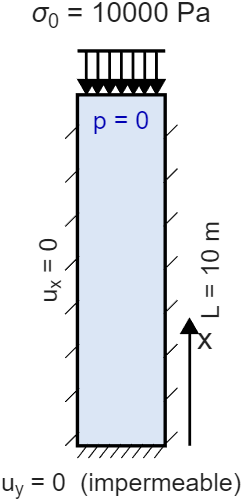
\includegraphics[width=0.20\textwidth]{tp3_esquema.png}
        \caption{Problema de Terzaghi: geometría, carga aplicada $\sigma_0$ en la
        cara superior drenante ($p=0$) y condiciones de borde de desplazamiento
        (caras laterales con $u_x=0$, base con $u_y=0$); todas las caras salvo la
        superior son impermeables. El eje $x$ mide la profundidad desde la base.}
        \label{fig:esquema}
    \end{figure}

    \begin{table}[H]
    \centering
    \resizebox{\columnwidth}{!}{%
    \begin{tabular}{lccc}
    \toprule
    \textbf{Propiedad} & \textbf{Símbolo} & \textbf{Set 1} & \textbf{Set 2} \\
    \midrule
    1er parámetro de Lamé [Pa] & $\lambda$ & $4.0\times10^{7}$ & $4.0\times10^{7}$ \\
    Módulo de corte [Pa]       & $\mu$     & $4.0\times10^{7}$ & $4.0\times10^{7}$ \\
    Coeficiente de Biot [-]    & $\alpha$  & $0.4$ & $0.4$ \\
    Módulo de Biot [Pa]        & $M$       & $4.1667\times10^{7}$ & $6.06\times10^{9}$ \\
    Porosidad [-]              & $\phi$    & $0.375$ & $0.375$ \\
    Permeabilidad [m$^2$]      & $k$       & $1.01937\times10^{-9}$ & $1.01937\times10^{-9}$ \\
    Viscosidad [Pa$\cdot$s]    & $\mu_f$   & $1.0$ & $1.0$ \\
    \bottomrule
    \end{tabular}%
    }
    \caption{Propiedades de los materiales para los dos sets analizados
    \cite{cheng2016}.}
    \label{tab:props}
    \end{table}

    \subsection{Formulación poroelástica y discretización}
    \quad El problema se gobierna por el balance de momento y el balance de masa de
    Biot \cite{biot1941}:
    \begin{equation}
    \nabla\!\cdot\!\bm{\sigma}=\bm{0},\qquad
    \bm{\sigma}=\mathbb{C}:\bm{\varepsilon}(\bm{u})-\alpha\,p\,\bm{I},
    \end{equation}
    \begin{equation}
    \frac{1}{M}\frac{\partial p}{\partial t}
    +\alpha\,\nabla\!\cdot\!\frac{\partial \bm{u}}{\partial t}
    -\nabla\!\cdot\!\Big(\frac{k}{\mu_f}\nabla p\Big)=0 .
    \end{equation}
    La discretización por elementos finitos \cite{bathe2006} conduce al sistema
    acoplado en las incógnitas nodales de desplazamiento $\bm{u}$ y presión
    $\bm{p}$:
    \begin{equation}
    \begin{bmatrix} \bm{K} & -\bm{Q}\\[2pt] \tfrac{1}{\Delta t}\bm{Q}^{\!\top} & \tfrac{1}{\Delta t}\bm{S}+\bm{H}\end{bmatrix}
    \!\begin{bmatrix}\bm{u}^{n+1}\\[2pt]\bm{p}^{n+1}\end{bmatrix}
    =\begin{bmatrix}\bm{F}\\[2pt]\bm{r}^{n}\end{bmatrix}
    \label{eq:monolitico}
    \end{equation}
    donde 
    \begin{itemize}
    \item$\bm{r}^{n}=\tfrac{1}{\Delta t}(\bm{S}\bm{p}^{n}+\bm{Q}^{\!\top}\bm{u}^{n})$
    \item $\bm{K}=\!\int\!\bm{B}^{\!\top}\mathbf{C}\bm{B}\,d\Omega$,
    \item$\bm{H}=\!\int\!(\nabla N_p)^{\!\top}\tfrac{k}{\mu_f}(\nabla N_p)\,d\Omega$,
    \item$\bm{Q}=\!\int\!\alpha\bm{B}^{\!\top}\!\bm{m}N_p\,d\Omega$
    \item$\bm{S}=\!\int\!\tfrac{1}{M}N_p^{\!\top}N_p\,d\Omega$. 
    \end{itemize}
    La integración temporal es
    de Euler implícita. Se emplea una malla de $2\times20$ elementos
    cuadriláteros \textbf{Q4} ($63$ nodos), donde desplazamiento y presión se
    interpolan con las mismas funciones de forma bilineales (igual orden), con
    $N_p$ los polinomios de los cuatro nodos del elemento. Se integra con
    cuadratura de Gauss de $2\times2$ puntos \cite{cook2002}.

    \subsection{Esquemas de acoplamiento y convergencia}
    \quad En lugar de resolver el sistema monolítico~\eqref{eq:monolitico}, se itera
    sobre sus bloques diagonales. El esquema \textit{staggered} resuelve, en cada
    iteración $k$ del paso temporal:
    \begin{align}
    \bm{K}\,\bm{u}^{(k)} &= \bm{F}+\bm{Q}\,\bm{p}^{(k-1)}, \\
    (\bm{S}+\Delta t\,\bm{H})\,\bm{p}^{(k)} &= \bm{S}\,\bm{p}^{n}-\bm{Q}^{\!\top}(\bm{u}^{(k)}-\bm{u}^{n}),
    \end{align}
    donde la ecuación de flujo se multiplicó por $\Delta t$. Su factor de
    contracción es $\rho_{\text{und}}=\alpha^2 M/K_{dr}$, con $K_{dr}=\lambda+2\mu$
    el módulo edométrico drenado; el esquema diverge cuando $\rho_{\text{und}}>1$.
    El \textit{fixed-stress split} \cite{mikelic2013} añade al paso de flujo una
    rigidez de estabilización $\bm{L}=(\alpha^2/K_{dr})\!\int\!N_p^{\top}N_p\,d\Omega$
    y lo resuelve primero:
    \begin{equation}
    \begin{aligned}
    (\bm{S}+\bm{L}+\Delta t\,\bm{H})\,\bm{p}^{(k)} ={}& \bm{S}\,\bm{p}^{n}+\bm{L}\,\bm{p}^{(k-1)} \\
    &-\,\bm{Q}^{\!\top}(\bm{u}^{(k-1)}-\bm{u}^{n}),
    \end{aligned}
    \end{equation}
    seguido del paso mecánico. Su contracción
    $\rho_{fs}=\alpha^2 M/(K_{dr}+\alpha^2 M)<1$ es incondicionalmente estable. En
    ambos casos el proceso iterativo se detiene cuando el incremento relativo de
    presión cumple
    \begin{equation}
    \frac{\lVert \bm{p}^{(k)}-\bm{p}^{(k-1)}\rVert_2}{\max\!\big(\lVert \bm{p}^{(k)}\rVert_2,\,1\big)} < \text{tol}.
    \end{equation}

    \quad La condición inicial no drenada se obtiene analíticamente: la carga
    instantánea genera una presión uniforme
    $p_0=\alpha M \sigma_0/(K_{dr}+\alpha^2 M)$ y un campo de desplazamiento
    $\bm{u}(x,0)$ resuelto del equilibrio mecánico $\bm{K}\bm{u}=\bm{F}+\bm{Q}\bm{p}_0$.
    Se comparan los resultados con la solución analítica en serie de Terzaghi
    \cite{terzaghi1943}, \begin{equation}p(x,t)=p_0\frac{4}{\pi}\sum_{m=0}^{\infty}\frac{(-1)^m}{2m+1}\cos(\lambda_m x)e^{-\lambda_m^2 c_v t}\end{equation}
    con $\lambda_m=(2m+1)\pi/2L$ y coeficiente de consolidación
    $c_v=(k/\mu_f)/(1/M+\alpha^2/K_{dr})$. Se realizan tres casos de análisis con los esquemas enunciados: 
    \begin{itemize}
        \item Solución con algoritmo \textit{staggered} del Set 1 hasta $t=\SI{6000}{s}$ ($\Delta t=\SI{1}{s}$)
        \item Solución con algoritmo \textit{staggered} del Set 2 hasta $t=\SI{600}{s}$ ($\Delta t=\SI{0.1}{s}$)
        \item Solución con algoritmo \textit{fixed-stress split} del Set 2 hasta $t=\SI{600}{s}$
    \end{itemize}

    \section{Resultados y Análisis}
    \quad La Tabla~\ref{tab:derivados} resume los parámetros adimensionales y los
    resultados de convergencia de cada caso. El cociente de acoplamiento
    $\alpha^2 M/K_{dr}$ predice correctamente la estabilidad del esquema
    \textit{staggered}: $0.056\ll1$ para el Set 1 y $8.08\gg1$ para el Set 2.

    \begin{table}[H]
    \centering
    \resizebox{\columnwidth}{!}{%
    \begin{tabular}{lcc}
    \toprule
    \textbf{Parámetro} & \textbf{Set 1} & \textbf{Set 2} \\
    \midrule
    $K_{dr}=\lambda+2\mu$ [Pa]       & $1.2\times10^{8}$ & $1.2\times10^{8}$ \\
    $c_v$ [m$^2$/s]                  & $0.0402$ & $0.680$ \\
    $p_0$ (no drenada) [Pa]          & $1316$ & $22247$ \\
    $\alpha^2 M/K_{dr}$ [-]          & $0.056$ & $8.08$ \\
    $\rho_{fs}$ [-]                  & --- & $0.890$ \\
    \midrule
    Iteraciones medias (\textit{stag.}) & $5.06$ & diverge \\
    Iteraciones medias (\textit{fixed-stress}) & --- & $2.05$ \\
    \bottomrule
    \end{tabular}%
    }
    \caption{Parámetros derivados y desempeño de los esquemas de acoplamiento. El
    \textit{staggered} del Set 2 diverge ($\alpha^2M/K_{dr}>1$); el
    \textit{fixed-stress} converge en $\sim2$ iteraciones (tol $=10^{-6}$).}
    \label{tab:derivados}
    \end{table}

    \subsection{Algoritmo \textit{staggered}, Set 1}
    \quad Con acoplamiento débil el esquema \textit{staggered} converge en
    promedio en $5.06$ iteraciones por paso. La Fig.~\ref{fig:tabla1} muestra un
    acuerdo prácticamente exacto entre la solución de elementos finitos (marcadores)
    y la analítica (líneas de trazos) en distintos instantes. Se observa la disipación
    progresiva de la sobrepresión desde la cara drenante ($x=L$) hacia la base
    impermeable. Como el asentamiento total está dominado por la respuesta
    instantánea no drenada y varía poco en el tiempo, se grafica el incremento de
    asentamiento por consolidación $u_y(t)-u_y(0)$ respecto del estado no drenado,
    que crece monótonamente y es máximo en la cara superior a medida que avanza la
    consolidación.

    \begin{figure}[H]
        \centering
        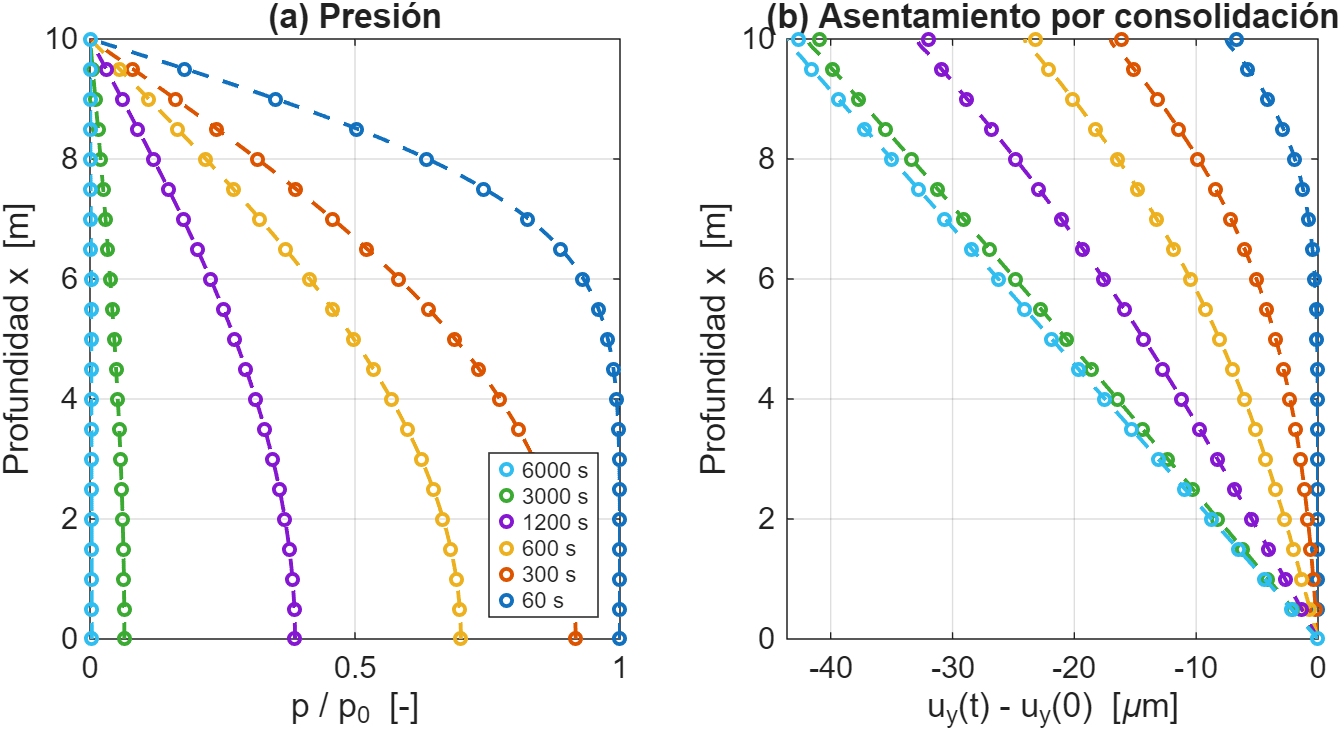
\includegraphics[width=0.48\textwidth]{tp3_tabla1.png}
        \caption{Set 1, esquema \textit{staggered} ($\Delta t=\SI{1}{s}$). (a)
        Presión normalizada $p/p_0$ y (b) incremento de asentamiento por
        consolidación $u_y(t)-u_y(0)$ respecto del estado no drenado, en función
        de la profundidad $x$, para $t=\{60,300,600,1200,3000,6000\}$ s. Marcadores:
        FEM; líneas de trazos: solución analítica \cite{terzaghi1943}.}
        \label{fig:tabla1}
    \end{figure}

    \subsection{Algoritmo \textit{staggered}, Set 2 (divergencia)}
    \quad Para el Set 2, con $\alpha^2 M/K_{dr}=8.08$, el esquema \textit{staggered}
    es inestable. La Fig.~\ref{fig:divergencia} muestra la norma
    $\lVert \bm{p}^{(k)}\rVert_2$ en función de la iteración $k$ para los primeros
    pasos temporales: en lugar de converger, la presión crece exponencialmente
    (nótese la escala logarítmica), alcanzando valores no físicos del orden de
    $10^{250}$ y produciendo el desbordamiento numérico de la solución en el paso 7
    ($t=\SI{0.7}{s}$). Como se detalla en la sección de convergencia, el
    desbordamiento ocurre en el paso 7 \emph{independientemente} de $\Delta t$:
    reducir el paso temporal no estabiliza el \textit{undrained split}, ya que la
    divergencia la gobierna el cociente $\alpha^2 M/K_{dr}>1$, que no depende de
    $\Delta t$.

    \begin{figure}[H]
        \centering
        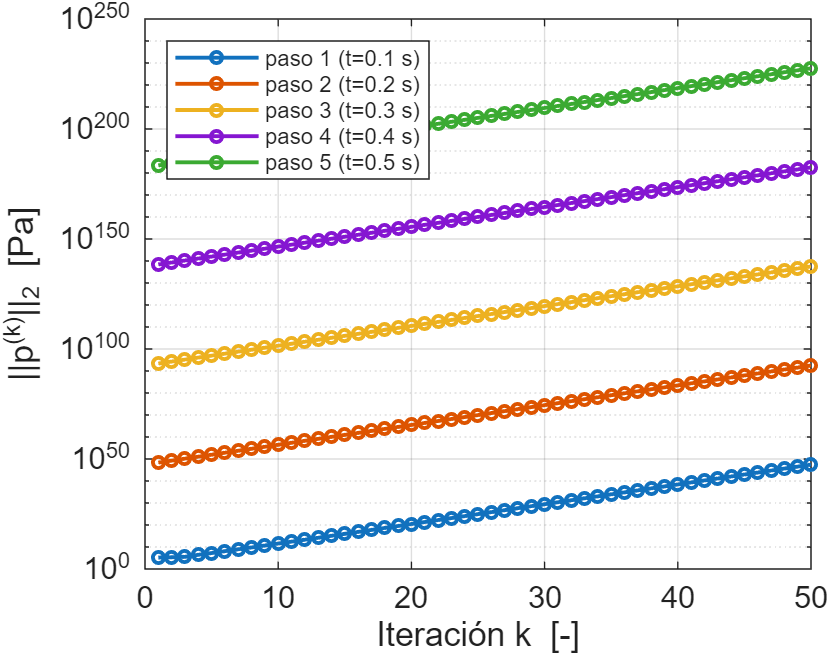
\includegraphics[width=0.42\textwidth]{tp3_divergencia.png}
        \caption{Set 2, esquema \textit{staggered} ($\Delta t=\SI{0.1}{s}$). Norma
        $\lVert \bm{p}^{(k)}\rVert_2$ [Pa] frente a la iteración $k$ para los
        primeros cinco pasos temporales (escala log). El crecimiento monótono
        evidencia la divergencia del esquema para $\alpha^2 M/K_{dr}>1$.}
        \label{fig:divergencia}
    \end{figure}

    \subsection{Algoritmo \textit{fixed-stress split}, Set 2}
    \quad Al estabilizar el paso de flujo con la rigidez $\bm{L}$, el
    \textit{fixed-stress split} recupera la estabilidad incondicional
    ($\rho_{fs}=0.890<1$). La Fig.~\ref{fig:fixedstress} muestra que la presión
    calculada reproduce con precisión la solución analítica para el mismo set de
    parámetros que hacía divergir al \textit{staggered}, requiriendo apenas $\sim2$
    iteraciones por paso (Tabla~\ref{tab:derivados}). El mayor coeficiente de
    consolidación del Set 2 ($c_v=0.68$~m$^2$/s frente a
    $0.04$~m$^2$/s del Set 1) explica la disipación mucho más rápida de la
    sobrepresión, esencialmente completa hacia $t=\SI{300}{s}$.

    \begin{figure}[H]
        \centering
        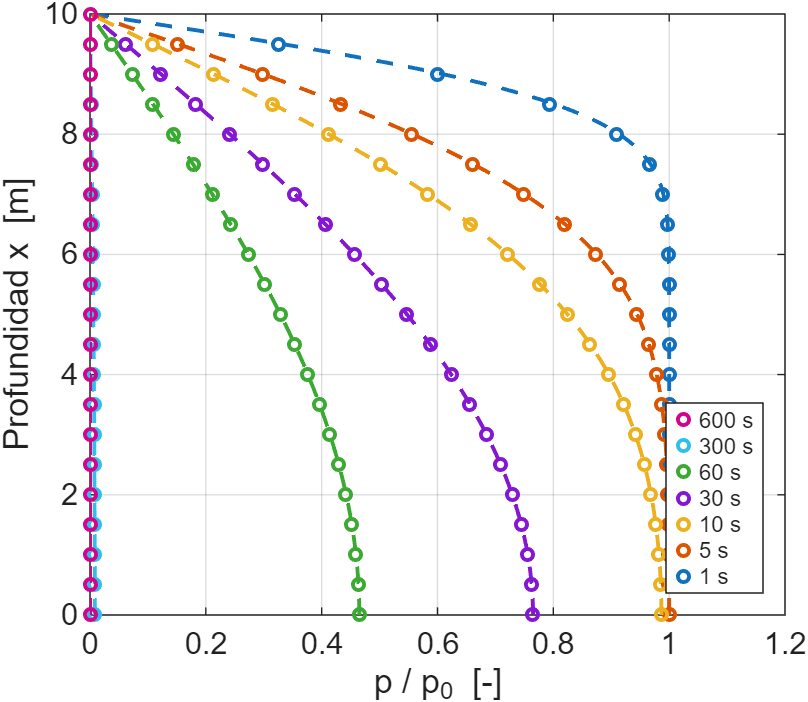
\includegraphics[width=0.42\textwidth]{tp3_fixedstress.png}
        \caption{Set 2, esquema \textit{fixed-stress split} ($\Delta t=\SI{0.1}{s}$).
        Presión normalizada $p/p_0$ frente a la profundidad $x$ para
        $t=\{1,5,10,30,60,300,600\}$ s. Marcadores: FEM; líneas de trazos: solución
        analítica \cite{terzaghi1943}.}
        \label{fig:fixedstress}
    \end{figure}

    \subsection{Análisis de convergencia y error}
    \quad Se cuantifica la precisión con el error relativo
    $\varepsilon=\max_x|p_{\text{FEM}}-p_{\text{anal}}|/p_0$ sobre la línea central.
    En la malla base ($20\times2$, $\Delta t=\SI{1}{s}$) resulta $\varepsilon=0.23\%$
    a $t=\SI{60}{s}$ y $0.05\%$ a $t=\SI{300}{s}$, cuantificando el acuerdo de la
    Fig.~\ref{fig:tabla1}.

    \quad La Fig.~\ref{fig:conv} resume los estudios de convergencia (Set 1, esquema
    estable). En el estudio \textbf{temporal} (a), con malla fija $100\times10$ y
    $\Delta t=\{2,1,0.5,0.25\}$ s, el error frente a la analítica decrece con
    pendiente $\approx1$, acorde al orden $\mathcal{O}(\Delta t)$ del esquema de
    Euler implícito. En el estudio \textbf{espacial} (b), para aislar el error de
    malla se compara cada malla con una solución de referencia en malla fina
    ($400\times40$) calculada con el mismo $\Delta t$, de modo que el error temporal
    es común y se cancela (comparar contra la analítica dejaría que el piso temporal
    enmascarara las dos mallas más finas). Refinando
    $20\times2\to100\times10\to200\times20$ el error decrece monótonamente con
    pendiente $\approx2.1$, en excelente acuerdo con el orden teórico
    $\mathcal{O}(h^2)$ de los elementos Q4. La malla base reproduce la analítica con
    error inferior al $0.25\%$, por lo que resulta adecuada para los análisis.

    \quad Para el Set 2 se verificó que la divergencia del \textit{staggered} es
    \emph{independiente de} $\Delta t$: para $\Delta t=\{0.2,0.1,0.05,0.01\}$ s la
    iteración interna nunca converge y la solución desborda siempre en el paso 7
    (antes en tiempo físico cuanto menor es $\Delta t$). La estabilidad la fija
    $\alpha^2M/K_{dr}$, no el paso temporal.

    \begin{figure}[H]
        \centering
        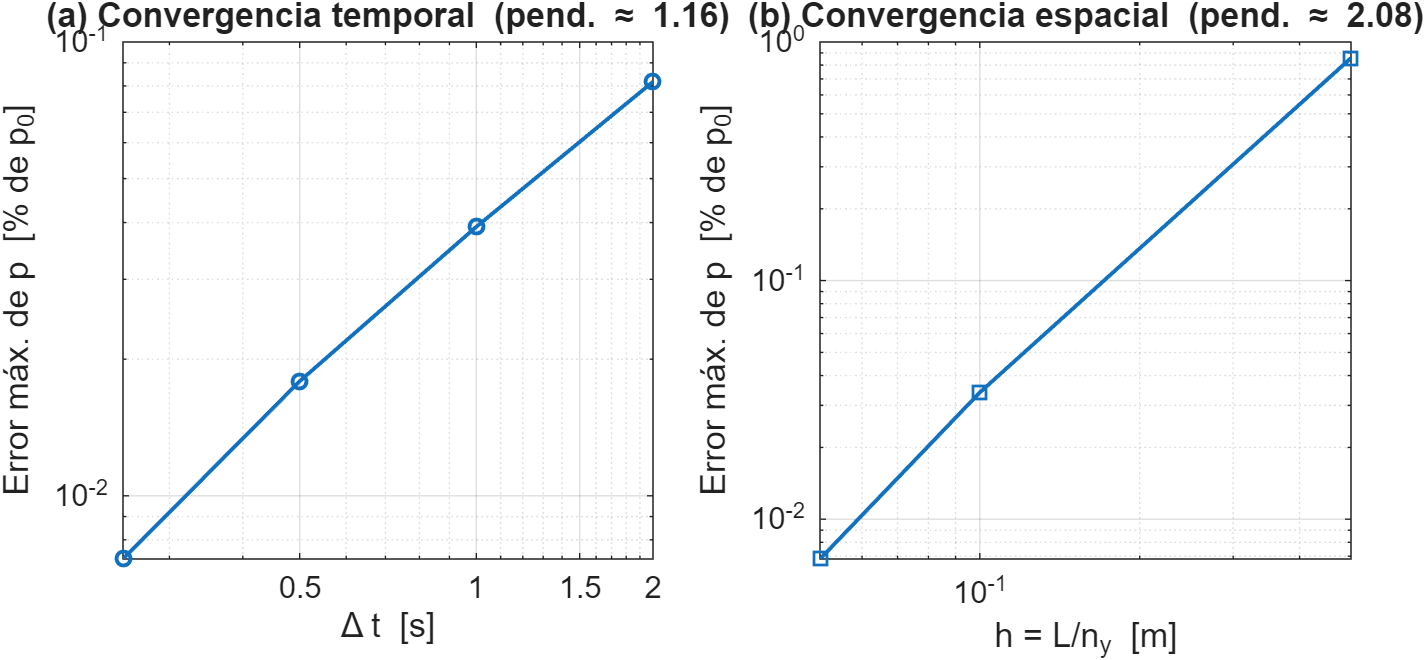
\includegraphics[width=0.48\textwidth]{tp3_convergencia.png}
        \caption{Estudios de convergencia (Set 1, \textit{staggered}), error máximo
        de presión en \% de $p_0$. (a) Convergencia temporal vs $\Delta t$ frente a
        la analítica (malla $100\times10$, $t=\SI{300}{s}$): pendiente $\approx1$,
        orden $\mathcal{O}(\Delta t)$. (b) Convergencia espacial vs $h=L/n_y$,
        error respecto de una solución de referencia $400\times40$
        ($\Delta t=\SI{0.5}{s}$, $t=\SI{30}{s}$): pendiente $\approx2.1$, orden
        $\mathcal{O}(h^2)$ de los elementos Q4.}
        \label{fig:conv}
    \end{figure}

    \quad El \textit{fixed-stress split} (Set 2) presenta el mismo comportamiento de
    convergencia (Fig.~\ref{fig:convfs}): orden temporal $\mathcal{O}(\Delta t)$
    (pendiente $\approx1.0$) y espacial $\mathcal{O}(h^2)$ (pendiente $\approx2.1$,
    error respecto de la referencia $400\times40$). Esto confirma que la
    estabilización del esquema no degrada la precisión de la solución.

    \begin{figure}[H]
        \centering
        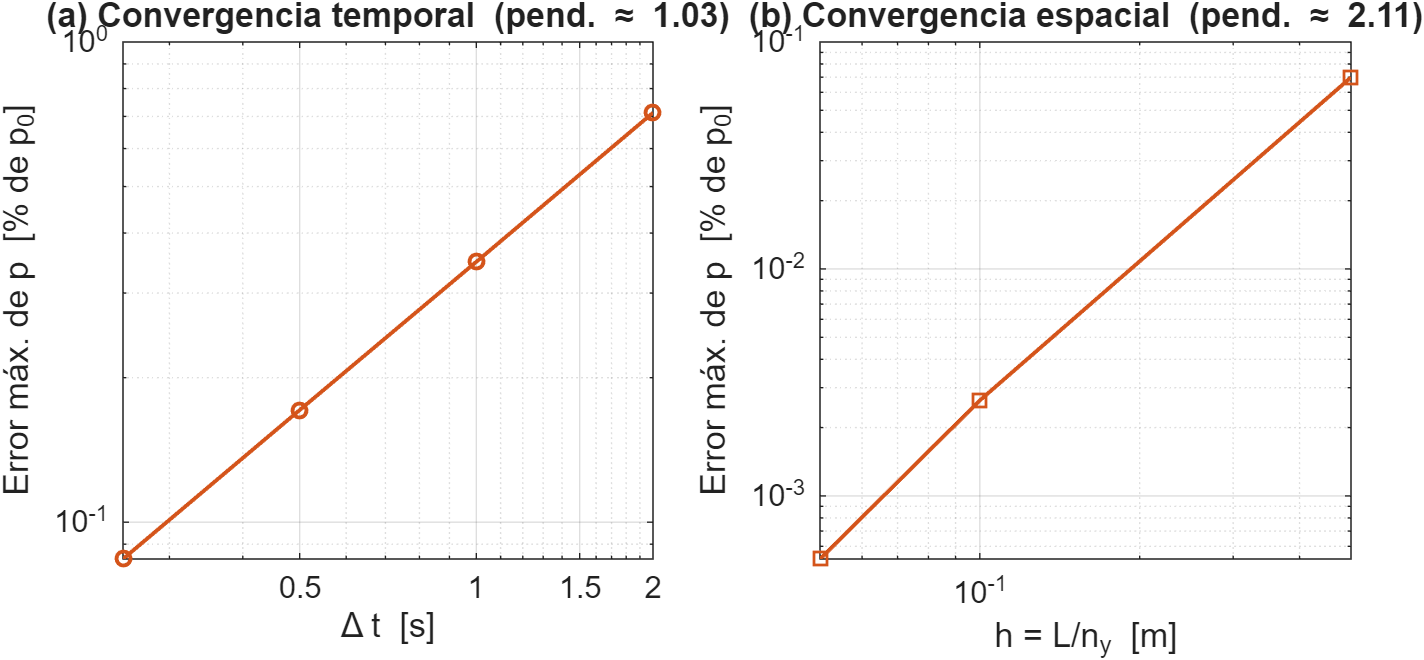
\includegraphics[width=0.48\textwidth]{tp3_convergencia_fs.png}
        \caption{Estudios de convergencia del \textit{fixed-stress split} (Set 2),
        error máximo de presión en \% de $p_0$. (a) Convergencia temporal vs
        $\Delta t$ frente a la analítica (malla $100\times10$, $t=\SI{30}{s}$):
        pendiente $\approx1$, orden $\mathcal{O}(\Delta t)$. (b) Convergencia
        espacial vs $h=L/n_y$, error respecto de una solución de referencia
        $400\times40$ ($\Delta t=\SI{0.5}{s}$, $t=\SI{30}{s}$): pendiente
        $\approx2.1$, orden $\mathcal{O}(h^2)$.}
        \label{fig:convfs}
    \end{figure}

    \section{Conclusiones}
    \quad Se cumplió el objetivo: se resolvió el problema de Terzaghi con una
    formulación poroelástica de Biot y se contrastaron los esquemas de acoplamiento.
    El esquema \textit{staggered} reproduce con exactitud la solución analítica
    cuando el acoplamiento es débil (Set 1, $\alpha^2 M/K_{dr}=0.056$), pero diverge
    de forma irrecuperable cuando es fuerte (Set 2, $\alpha^2 M/K_{dr}=8.08$),
    independientemente del paso temporal. El \textit{fixed-stress split} resuelve
    esta limitación: es incondicionalmente estable ($\rho_{fs}=0.890$) y converge en
    $\sim2$ iteraciones por paso, reproduciendo la solución analítica para el caso
    fuertemente acoplado. Los estudios de convergencia confirman el orden temporal
    $\mathcal{O}(\Delta t)$ y espacial $\mathcal{O}(h^2)$ esperados, siendo la malla
    base suficiente (error $<0.25\%$ frente a la analítica). Por último se concluyó que el
    cociente $\alpha^2 M/K_{dr}$ resultó un predictor fiable de la estabilidad del
    \textit{undrained split}, independiente de $\Delta t$.

    \printbibliography

    \end{document}
